\chapter{Automatic Differentiation}
% Authors: Joanna Bitton, Divyansh Khanna, Lind Xiao, 2/26/19.
Automatic differentiation is a hybrid of symbolic differentiation and numerical differentiation.
It is extremely efficient when it is desired to differentiate functions of the form
$$y_n=f_n(w_{n-1}, f_{n-1}(w_{n-2},\cdots (f_0(w_0, x_0)) $$
When back-propagation is performed, there is a desire that $\partial y_{k}/\partial w_{\ell}$ can be explicitly expressed in terms of $y_k$.
Thankfully, there are packages that handle auto-differentiation such that it does not have to be done manually.

In \texttt{pytorch}, each tensor has an attribute called \texttt{grad\_fn} which handles the process of calculating $\partial y/\partial x$ with a given $y$.
Note that \texttt{grad\_fn=None} for those tensors that cannot be differentiated.
For each derived tensor, \texttt{pytorch} internally builds a computation graph.
Moreover, gradients can be constructed implicitly with the \texttt{backward()} method.

For both memory and efficiency reasons, the computation graph would be discarded once it is backwarded.
By default, a computation graph can not be backwarded twice.
Once the parameters are updated, the backwarded scalar must be recomputed before the computation graph can be constructed at a new position.

In general the \texttt{backward()} method requires an input of the same size as the backwarded tensor.
\begin{minted}{python}
y.backward(h)
# h * J(x)  = x.grad, where J(x) is the Jacobian calculated from y
# though pytorch does not calculate and store Jacobian internally
\end{minted}

By default, explicitly constructed tensor \texttt{x}
has \texttt{x.require\_grad=False}.
The \texttt{require\_grad} attribute can be manually turned on or off for leaf nodes on the computation graph (they do not depend on another tensor).
If it is desired to turn off a \texttt{requires\_grad} for an intermediate result, it must be copied and without reference.
The \texttt{.detach()} method is handy for this purpose.
\begin{minted}{python}
n = 3
x = torch.randn(n, requires_grad=True)
w = torch.ones(n, requires_grad=True)

z = w @ x

z1 = z.detach()

z2 = w * z1 @ x;
z2.backward()
print(w.grad, z1.grad, x.grad, sep='\n')
\end{minted}
The output would be:
\begin{minted}{python}
tensor([-0.2010, -0.0613,  0.5340])
None
tensor([0.5213, 0.5213, 0.5213])
\end{minted}

\chapter{Random Projections}
% Authors: Joanna Bitton, Divyansh Khanna, Lind Xiao, 2/26/19.
The dimensionality of data significantly impacts how well a machine learning model can generalize.
Consider unit orthogonal vectors in space.
With increasing dimensions, the number of orthogonal vectors increase exponentially (\href{https://www.cs.princeton.edu/courses/archive/fall15/cos521/lecnotes/lec12.pdf}{source}).
To generalize well, the model needs at least \texttt{exp(d)} points, where \texttt{d} is the data dimension.
This is because for a new data point, the models should find another point in the dataset which is reasonably close to it. 

The \href{https://github.com/Atcold/pytorch-Deep-Learning-Minicourse/blob/master/extra/a-projections.ipynb}{Jupyter notebook} illustrates orthogonality of random projections using a simple example.
It plots the projection \texttt{p} of a random matrix \texttt{A} with one of its randomly chosen rows \texttt{a}.
Since \texttt{A} is a random matrix of unit vectors (normalized with unitary L-2 norm), \texttt{p} will have a value of \texttt{1} for one row. 

Figure 2 shows the matrix plots for \texttt{d=3}.
There are at least three rows in the projections which have a value greater than \texttt{0.800}.
Figure 3 shows the matrix plots for \texttt{d=5}.
There are no rows with a value close to \texttt{1}, except for the one corresponding to \texttt{a}.

The intuition is that in low dimensions random vectors point roughly in same directions.
However in high dimensions, they point orthogonal to each other.
As the dimensionality of the data is increased, more points becomes further apart and there are less matches.

\begin{figure}
    \centering
    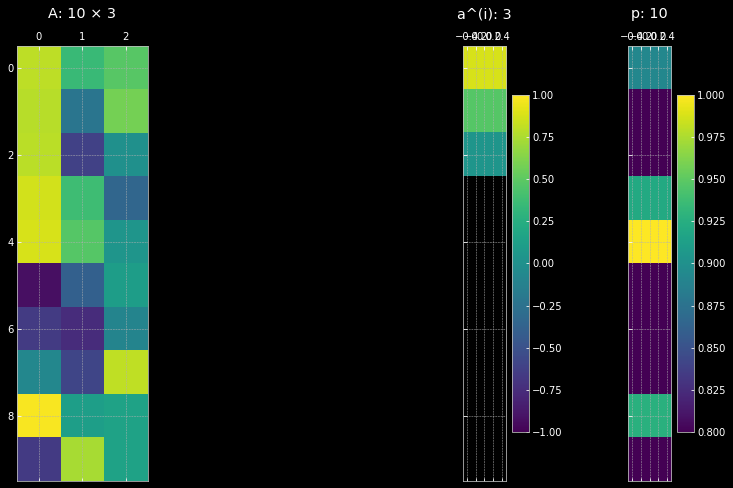
\includegraphics[width=0.85\textwidth]{labs/05/images/dim3.png}
    \caption{Projecting p for A with dimensions (10, 3)}
    \label{fig:my_label1}
    \vspace{5mm}
    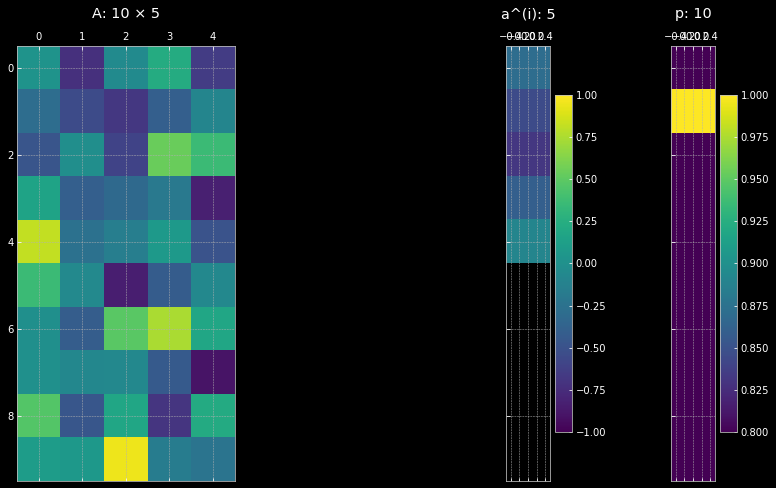
\includegraphics[width=0.85\textwidth]{labs/05/images/dim5.png}
    \caption{Projecting p for A with dimensions (10, 5)}
    \label{fig:my_label2}
\end{figure}